From applying the pipeline we have just discussed, we obtained the following hyper-parameters for Ridge Regressor
\begin{itemize}
    \item $n_{RI} = 50$
    \item \textit{alpha}: 2
    \item \textit{fit\_intercept}: \textit{True}
    \item \textit{max\_iter}: \textit{None}
\end{itemize}
while for the MLP Regressor the hyper-parameters are
\begin{itemize}
    \item $n_{MLP} = 40$
    \item \textit{hidden\_layer\_sizes}: (100,)
    \item \textit{activation}: \textit{logistic}
    \item \textit{solver}: \textit{adam}
    \item \textit{alpha}: 1
    \item \textit{max\_iter}: 1000
\end{itemize}


Once defined the quantities $n_{RI}$ and $n_{MLP}$ and tuned the hyper-parameters using a portion of the development set, we validated the resultant regressors on the other part of the dataset.

A first analysis of the performance of the model can be done by looking at the residuals, that is the quantity $\epsilon_i = y_i - \hat{y_i}$. 
Theoretically, they should represent the white noise in data and thus should be distributed as
$$\epsilon_i \overset{\text{iid}}{\sim} \mathcal{N}(0, \sigma^2)$$

Looking at the behaviour of the residuals we obtained, shown in \eqref{fig:res_Ridge} and \eqref{fig:res_MLP}, we can appreciate that they are distributed around the mean value 0 for both models, but the hypothesis of homoscedasticity is not satisfied. The cause could be a lacking representativeness of people over the age of 50 in the dataset, as noticed during the data exploration and confirmed by the fact that most of the residuals are positive, meaning that the two regressors often predict a smaller age when the true one is over 35.

Moreover, we sadly notice that the variance of the residuals is very large especially when predicting larger values of the response variable. Comparing the two plots, it has to be said that the MLP regressor is the one whose residuals have greater variance.

\begin{figure}
    \centering
    % First PDF image
    \begin{subfigure}{0.23\textwidth}
        \centering
        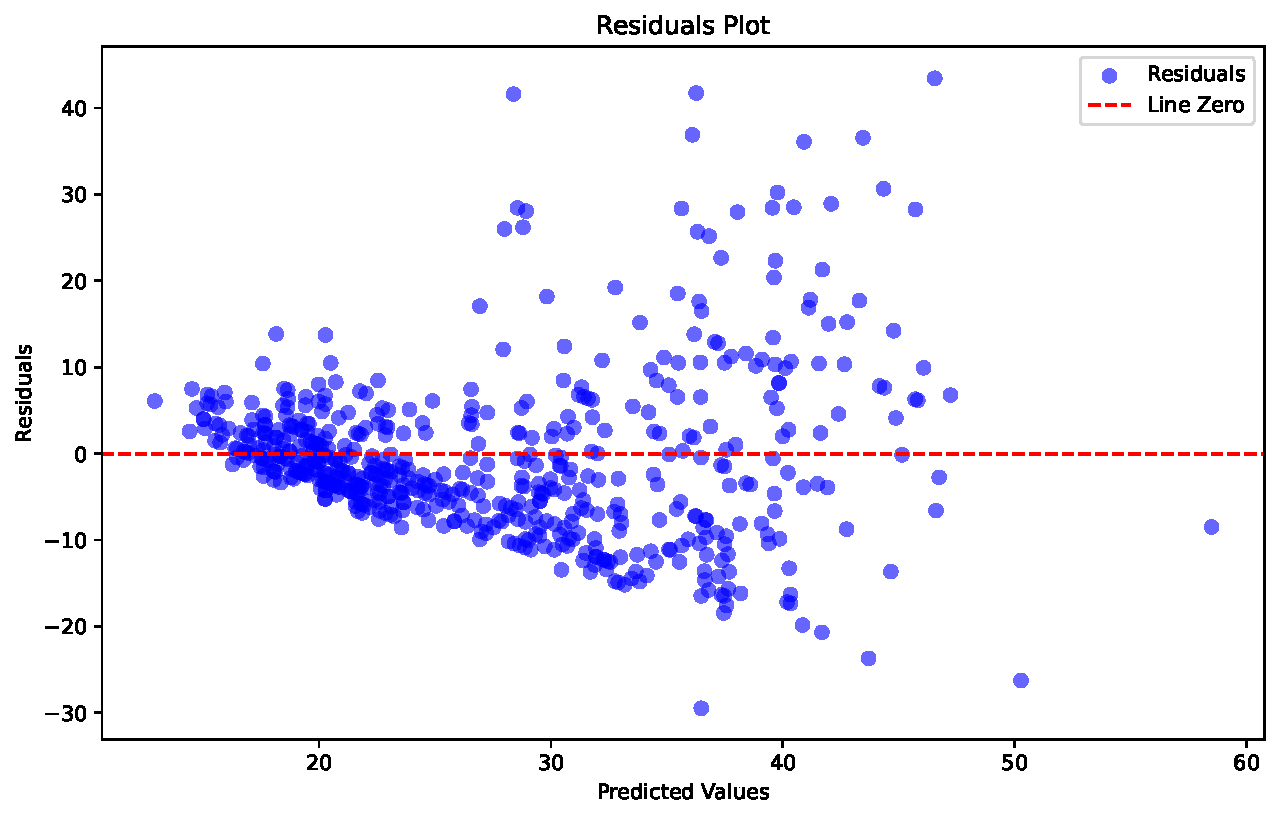
\includegraphics[width=\textwidth]{img/residuals_RI_1.pdf}
    \end{subfigure}
    % Second PDF image
    \begin{subfigure}{0.23\textwidth}
        \centering
        
\includegraphics[width=\textwidth]{img/residuals_RI_2.pdf} 
    \end{subfigure}
    \caption{Residuals plot and distribution for the Ridge Regressor}
    \label{fig:res_Ridge}
\end{figure}

\begin{figure}
    \centering
    % First PDF image
    \begin{subfigure}{0.23\textwidth}
        \centering
        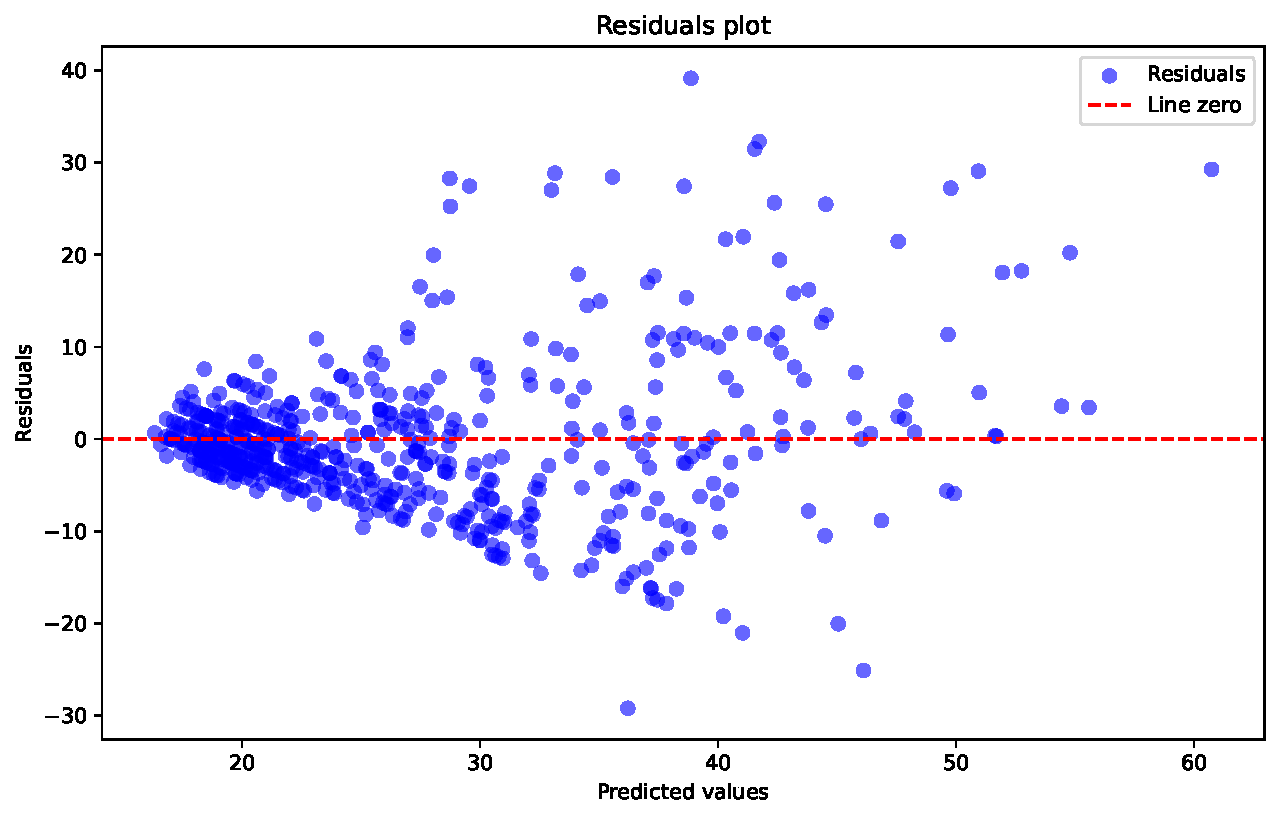
\includegraphics[width=\textwidth]{img/residuals_mlp_2.pdf}
    \end{subfigure}
    % Second PDF image
    \begin{subfigure}{0.23\textwidth}
        \centering
        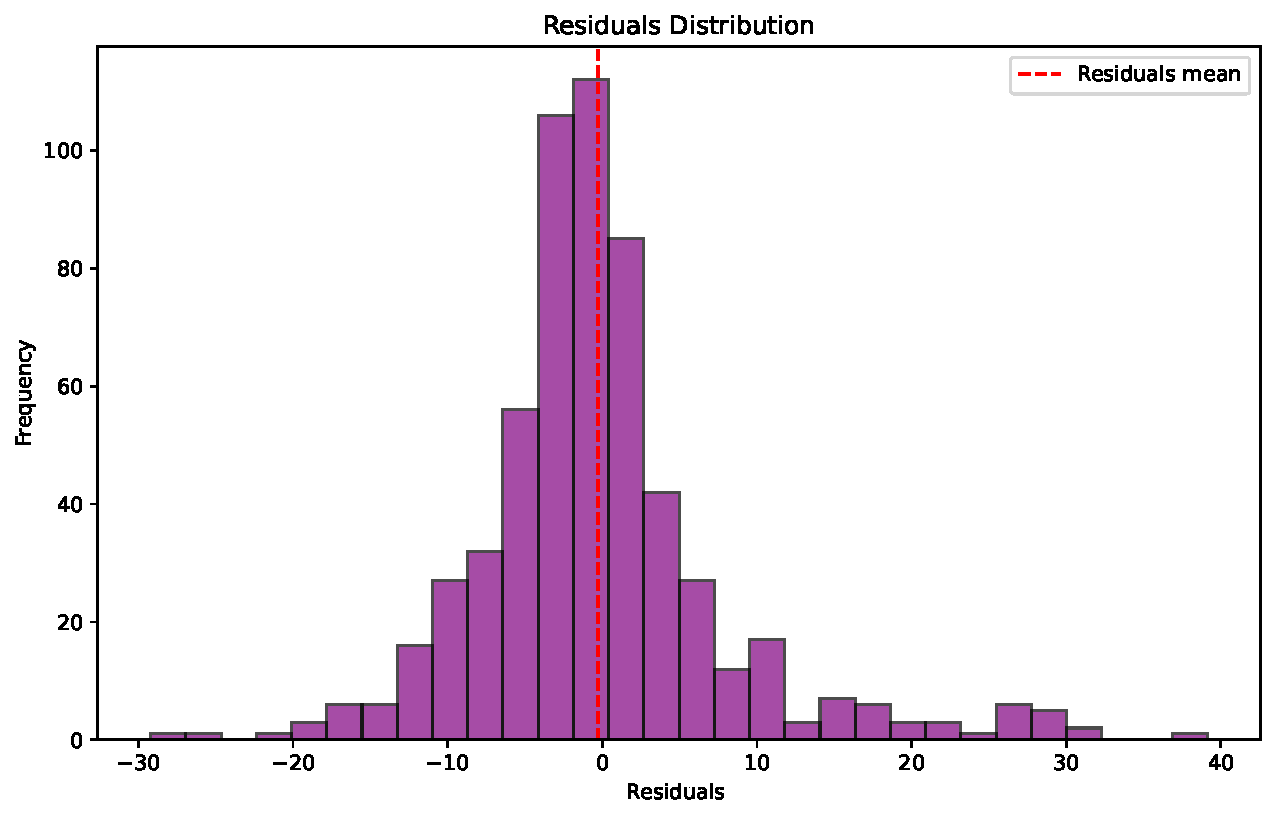
\includegraphics[width=\textwidth]{img/residuals_mlp_1.pdf} 
    \end{subfigure}
    \caption{Residuals plot and distribution for the MLP Regressor}
    \label{fig:res_MLP}
\end{figure}

During the phase of validation, we decided to evaluate the model not only in terms of RMSE but also by computing the $R^2$ score: the scores obtained are of 0.4520 for the Ridge regressor and of 0.3927 for the MLP regressor. The fact that the MLP Regressor is scored with a lower $R^2$ value restates what was shown in the residuals plots, that is that the MLP regressor residuals have higher variance.
This allows us to say that the solution we have found works slightly better than just predicting the mean value of the response variable. Still, they are pretty far from their maximum value 1 which means that the regressors fail to capture great part of the variance of the data.

The public score obtained is 9.974 for the Ridge Regressor and 9.726 for the MLP Regressor.
As these represent the first scores derived from the evaluation data, overfitting is unlikely, and it is reasonable to expect similar results on the private score.